% Created 2016-03-21 Mon 22:35
\documentclass[bigger]{beamer}
\usepackage[utf8]{inputenc}
\usepackage[T1]{fontenc}
\usepackage{fixltx2e}
\usepackage{graphicx}
\usepackage{longtable}
\usepackage{float}
\usepackage{wrapfig}
\usepackage{rotating}
\usepackage[normalem]{ulem}
\usepackage{amsmath}
\usepackage{textcomp}
\usepackage{marvosym}
\usepackage{wasysym}
\usepackage{amssymb}
\usepackage{hyperref}
\tolerance=1000
\usepackage{tikz}
\usepackage{minted}
\usemintedstyle{pastie}
\usetheme{default}
\author{Tobi Lehman}
\date{2016-03-02 Wed}
\title{Object Oriented Orbits: a primer on Newtonian physics}
\hypersetup{
  pdfkeywords={},
  pdfsubject={A tour through the mathematics, physics and source code required to simulate a universe with gravity.},
  pdfcreator={Emacs 24.5.1 (Org mode 8.2.10)}}
\begin{document}

\maketitle

\begin{frame}[label=sec-1]{What does it take to simulate orbits?}
\begin{center}
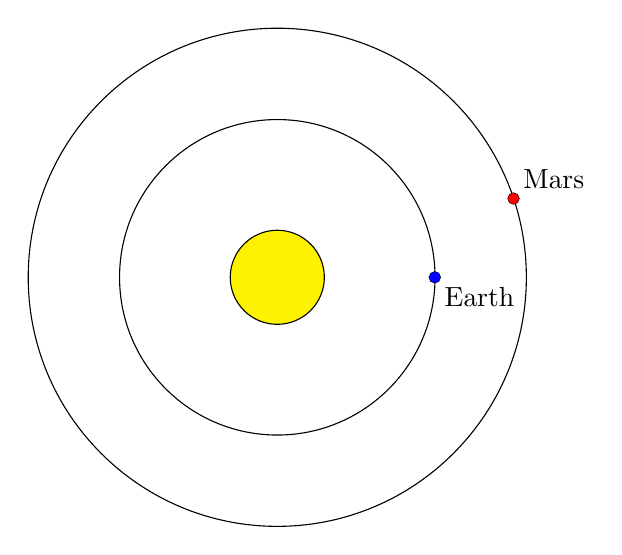
\begin{tikzpicture}
\coordinate (s) at (0,0);
\coordinate (e) at (2,0);
\coordinate (m) at (3,1);

\fill[yellow] (s) circle (17pt);
\draw[black] (s) circle (17pt);

\draw[black] (e) circle (2pt);
\draw[black] (s) circle  (57pt);
\node[below right] at (e) {Earth};
\fill[blue] (e) circle (2pt);

\draw[black] (m) circle (2pt);
\draw[black] (s) circle  (90pt);
\node[above right] at (m) {Mars};
\fill[red] (m) circle (2pt);
\end{tikzpicture}
\end{center}
\end{frame}

\begin{frame}[label=sec-2]{What we need}
\begin{block}{Before we can simulate orbits, we need to a few things}
\begin{itemize}
\item a \alert{model of space} to organize the simulated bodies
\item a \alert{dynamic rule} to update the locations of bodies in space
\end{itemize}
\end{block}
\end{frame}

\begin{frame}[label=sec-3]{Euclid's axioms}
\begin{block}{The first complete model of space ever recorded was compiled by Euclid in ancient Greece.}
\end{block}
\end{frame}

\begin{frame}[label=sec-4]{Axiom 1}
\begin{block}{Between any two points ${\color{red} A}$ and ${\color{blue} B}$, a line segment $L$ can be drawn}
\begin{center}
\begin{tikzpicture}
    \coordinate (a) at (0,0);
    \coordinate (b) at (5,1);
    \coordinate (L) at (2.5,0.5);
    \draw (a) to (b);
    \fill[red] (a) circle (2pt);
    \fill[blue] (b) circle (2pt);
    \node[below left] at (a) {A};
    \node[below right] at (b) {B};
    \node[above] at (L) {L};
\end{tikzpicture}
\end{center}
\end{block}
\end{frame}

\begin{frame}[label=sec-5]{Axiom 2}
\begin{block}{A line segment $L$ can be extended indefinitely to a larger line segment $L'$, that contains $L$}
\begin{center}
\begin{tikzpicture}
    \coordinate (a) at (0,0);
    \coordinate (b) at (5,1);
    \coordinate (L) at (2.5,0.5);
    \draw (a) to (b);
    \draw (-0.5,-0.1) to (5.5, 1.1);
    \fill[red] (a) circle (2pt);
    \fill[blue] (b) circle (2pt);
    \node[below left] at (a) {A};
    \node[below right] at (b) {B};
    \node[above] at (L) {L};
    \node[below right] at (L) {L'};
\end{tikzpicture}
\end{center}
\end{block}
\end{frame}
\begin{frame}[label=sec-6]{Axiom 3}
\begin{block}{A circle can be drawn at any point with any radius}
\begin{center}
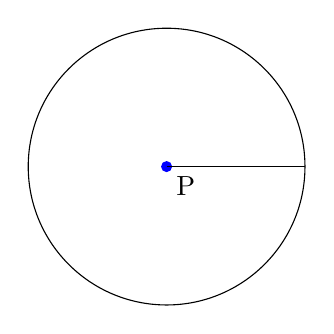
\begin{tikzpicture}
\coordinate (p) at (0,0);
\coordinate (rp) at (1.76,0);
\draw[black] (p) circle (50pt);
\fill[blue] (p) circle (2pt);
\node[below right] at (p) {P};
\draw (p) to (rp);
\end{tikzpicture}
\end{center}
\end{block}
\end{frame}

\begin{frame}[label=sec-7]{Axiom 4}
\begin{block}{All right angles are congruent}
\begin{center}
\begin{tikzpicture}
\coordinate (a) at (0,0);
\coordinate (b) at (0,1);
\coordinate (c) at (1,0);
\coordinate (b') at (0,2);
\coordinate (c') at (2,0);

\draw[red, ultra thick] (a) to (b);
\draw[red, ultra thick] (a) to (c);
\draw[blue] (a) to (b');
\draw[blue] (a) to (c');

\draw (a) rectangle (0.2,0.2);
\end{tikzpicture}
\end{center}
\end{block}
\end{frame}

\begin{frame}[label=sec-8]{Axiom 5 (The Parallel Postulate)}
\begin{block}{Given a line $L$ and a point $p$ not on the line, there is exactly one line $L'$ through $p$ that doesn't intersect $L$}
\begin{center}
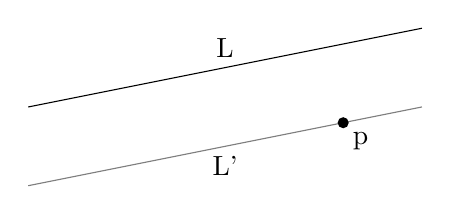
\begin{tikzpicture}
\coordinate (L1) at (0,0);
\coordinate (L2) at (5,1);
\coordinate (L1') at (0,-1);
\coordinate (L2') at (5,0);
\coordinate (L) at (2.5, 0.5);
\coordinate (L') at (2.5, -.5);
\coordinate (p) at (4,-0.2);

\draw (L1) to (L2);
\node[above] at (L) {L};
\node[below] at (L') {L'};
\fill[black] (p) circle (2pt);
\node[below right] at (p) {p};
\draw[opacity=0.5] (L1') to (L2');
\end{tikzpicture}
\end{center}
\end{block}
\end{frame}

\begin{frame}[label=sec-9]{Theorems}
\begin{block}{From these five axioms, we can deduce many useful things, the most useful for our purposes will be the Pythagorean theorem.}
\begin{center}
\begin{tikzpicture}
\coordinate (x) at (0,0);
\coordinate (y) at (0,3);
\coordinate (z) at (4,0);

\coordinate (A) at (0,1.5);
\coordinate (B) at (2,0);
\coordinate (C) at (1.5,2);

\draw[black] (x) to (y);
\draw[black] (x) to (z);
\draw[black] (y) to (z);

\draw (x) rectangle (0.5,0.5);
\node[left] at (A) {A};
\node[below] at (B) {B};
\node[right] at (C) {C};
\node[below] at (2,-1) {$A^2 + B^2 = C^2$};
\end{tikzpicture}
\end{center}
\end{block}

\begin{block}{We can use this to compute distance}
\end{block}
\end{frame}

\begin{frame}[label=sec-10]{Axioms 1 and 2 and vectors}
\begin{block}{Vectors are \alert{directed line segments}, which can be \alert{scaled by real numbers}, so axioms 1 and 2 are relevant for vectors}
\begin{enumerate}
\item Given any two points $A$ and $B$, a vector $\vec{v}$ exists whose tail is $A$ and head is $B$

\item Given any vector $\vec{v}$ and any real number $c$, $c\vec{v}$ extends $\vec{v}$ by a factor of $c$
\end{enumerate}

\begin{center}
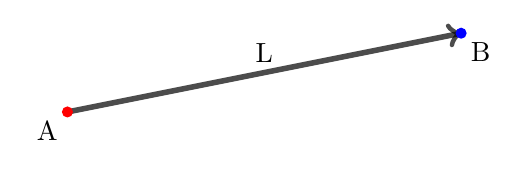
\begin{tikzpicture}
    \coordinate (a) at (0,0);
    \coordinate (b) at (5,1);
    \coordinate (L) at (2.5,0.5);
    \draw[->,line width=2,opacity=0.7] (a) to (b);
    \fill[red] (a) circle (2pt);
    \fill[blue] (b) circle (2pt);
    \node[below left] at (a) {A};
    \node[below right] at (b) {B};
    \node[above] at (L) {L};
\end{tikzpicture}
\end{center}
\end{block}
\end{frame}

\begin{frame}[label=sec-11]{Some terminology}
\begin{block}{We call the initial point of a vector its \alert{tail}}
\end{block}
\begin{block}{The final point of the vector is called its \alert{head}}
\begin{center}
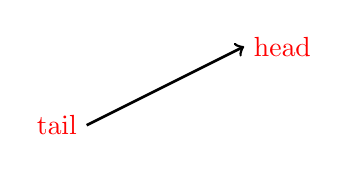
\begin{tikzpicture}
\coordinate (a) at (0,0);
\coordinate (b) at (2,1);
\draw[->,line width=1] (a) to (b);
\node[left,red] at (a) {tail};
\node[right,red] at (b) {head};
\end{tikzpicture}
\end{center}
\end{block}
\end{frame}
\begin{frame}[label=sec-12]{Vectors can be added}
\begin{block}{Given any two vectors $\vec{v}$ and $\vec{w}$ \uline{with the same tail}, their sum $\vec{v} + \vec{w}$ can be visualized using a parallelogram:}
\begin{center}
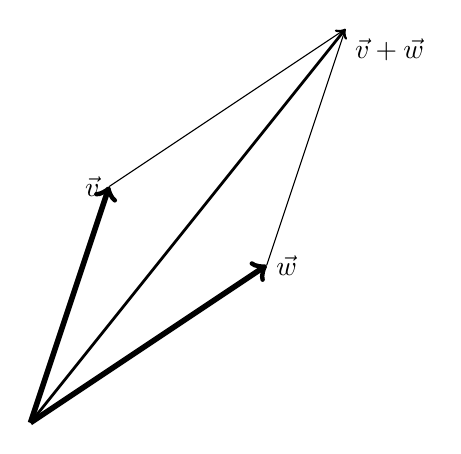
\begin{tikzpicture}
\coordinate (a) at (0,0);
\coordinate (b) at (3,2);
\coordinate (c) at (1,3);
\coordinate (b_c) at (4,5);


\draw[->,line width=2] (a) to (b);
\draw[->,line width=2] (a) to (c);
\draw[->,line width=1] (a) to (b_c);
\draw (b) to (b_c);
\draw (c) to (b_c);

\node[left] at (c) {$\vec{v}$};
\node[below right] at (b_c) {$\vec{v}+\vec{w}$};
\node[right] at (b) {$\vec{w}$};
\end{tikzpicture}
\end{center}
\end{block}

\begin{block}{This uses \alert{axiom 5}, and this operation is commutative}
\end{block}
\end{frame}

\begin{frame}[label=sec-13]{Vectors and coordinate systems}
\begin{block}{Given a coordinate system, we can represent vectors using pairs (2D) or triples (3D) of real numbers:}
\end{block}
\begin{block}{There is a special point, $\vec{0}$ which is just the origin.}
\begin{center}
\begin{tikzpicture}
% The axes
\draw[->] (xyz cs:x=-4) -- (xyz cs:x=4) node[above] {$x$};
\draw[->] (xyz cs:y=-4) -- (xyz cs:y=4) node[right] {$z$};
\draw[->] (xyz cs:z=-4) -- (xyz cs:z=4) node[above] {$y$};
% The thin ticks
\foreach \coo in {-4,-3,...,4}
{
  \draw (\coo,-1.5pt) -- (\coo,1.5pt);
  \draw (-1.5pt,\coo) -- (1.5pt,\coo);
  \draw (xyz cs:y=-0.15pt,z=\coo) -- (xyz cs:y=0.15pt,z=\coo);
}
% The thick ticks
\draw[thick] (3,-3pt) -- (3,3pt) node[below=6pt] {3};
\draw[thick] (-3pt,4) -- (3pt,4) node[left=6pt] {4};
\draw[thick] (xyz cs:y=-0.3pt,z=-2) -- (xyz cs:y=0.3pt,z=-2) node[below right=4pt] {-2};

\fill[blue] (2,3.5,-2) circle (2pt);
\node[left,color=blue] at (2,3.5,-2) {(2,3.5,-2)};
\draw[->,line width=1,color=red] (0,0,0) to (2,3.5,-2);

\end{tikzpicture}
\end{center}
\end{block}
\end{frame}
\begin{frame}[label=sec-14]{Vectors have a 'dot product'}
\begin{block}{Given any two vectors $\vec{v} = (v_1,v_2,v_3)$ and $\vec{w} = (w_1,w_2,w_3)$}
\end{block}
\begin{block}{their dot product $\vec{v} \cdot \vec{w} = v_1w_1 + v_2w_2 + v_3w_3$}
\end{block}
\begin{block}{\alert{Useful fact:} $\vec{v} \cdot \vec{w} = |v||w|cos(\theta)$}
\end{block}
\begin{block}{That also implies that $\sqrt{\vec{v} \cdot \vec{v}}$ is the length of the vector}
\end{block}
\end{frame}
\begin{frame}[label=sec-15]{Distance between vectors}
\begin{block}{We are using vectors to represent points in space, so we will compute the distance between the points $V$ and $W$ by computing $\sqrt{(\vec{v}-\vec{w})\cdot (\vec{v}-\vec{w})}$. \alert{This dot product magic just follows from the Pythagorean theorem}.}
\begin{center}
\begin{tikzpicture}
% The axes
\draw[->] (xyz cs:x=-3) -- (xyz cs:x=3) node[above] {$x$};
\draw[->] (xyz cs:y=-3) -- (xyz cs:y=3) node[right] {$z$};
\draw[->] (xyz cs:z=-3) -- (xyz cs:z=3) node[above] {$y$};
% The thin ticks
\foreach \coo in {-3,-2,...,3}
{
  \draw (\coo,-1.5pt) -- (\coo,1.5pt);
  \draw (-1.5pt,\coo) -- (1.5pt,\coo);
  \draw (xyz cs:y=-0.15pt,z=\coo) -- (xyz cs:y=0.15pt,z=\coo);
}
% The thick ticks

\draw[->,line width=1,color=black] (0,0,0) to (2,1,-1);
\node[right] at (2,1,-1) {$\vec{w}$};
\draw[->,line width=1,color=black] (0,0,0) to (-2,2,1);
\node[left] at (-2,2,1) {$\vec{v}$};
\node[above] at (-0.5,2,1) {$\vec{v}-\vec{w}$};

\draw[style=dashed] (2,1,-1) to (-2,2,1);
\end{tikzpicture}
\end{center}
\end{block}
\end{frame}

\begin{frame}[fragile,label=sec-16]{Vectors in Ruby (components)}
 \begin{block}{Now that we have a \alert{model of space}, we can start writing some ruby code}
\begin{itemize}
\item a Vector has components (the coordinates)
\end{itemize}
\begin{minted}[]{ruby}
class Vector
  attr_reader :components

  def initialize(components)
    @components = components
  end
end
\end{minted}
\end{block}
\end{frame}

\begin{frame}[fragile,label=sec-17]{Vectors in Ruby (algebra)}
 \begin{itemize}
\item a Vector can be added to another vector
\item a Vector can be multiplied by a scalar
\end{itemize}
\begin{minted}[]{ruby}
class Vector
  def +(vector)
    sums = components.zip(vector.components).
                      map {|(vi,wi)| vi+wi }
    Vector.new(sum)
  end

  def *(scalar)
    Vector.new(components.map{|c| scalar*c })
  end
end
\end{minted}
\end{frame}

\begin{frame}[fragile,label=sec-18]{Vectors in Ruby (equality and dot product)}
 \begin{itemize}
\item we can compare two vectors for equality
\item we can take the dot product of two vectors and get the scalar
\end{itemize}

\begin{minted}[]{ruby}
class Vector
  def ==(vector)
    components == vector.components
  end

  def dot(vector)
    pairs = components.zip(vector.components)
    pairs.map {|(vi,wi)| vi*wi }.
          inject(&:+)
  end
end
\end{minted}
\end{frame}
\begin{frame}[label=sec-19]{Time}
\begin{block}{Now we have a decent \alert{model of space}, we can move on to the \alert{dynamic rule}, it will be a way to update the state of the bodies in space over time.}
\end{block}
\end{frame}
\begin{frame}[label=sec-20]{Relation between position, time and velocity}
\begin{block}{We can represent the path a body takes using a function $\vec{x}(t)$.}
\end{block}

\begin{block}{The velocity is then just the \alert{rate of change of position with respect to time}}
\begin{center}
{\LARGE $\vec{v}(t) = \frac{d\vec{x}}{dt}$}
\end{center}
\end{block}
\end{frame}

\begin{frame}[label=sec-21]{Relation between velocity and acceleration}
\begin{block}{Similarly, the acceleration is the \alert{rate of change of velocity with respect to time}}
\begin{center}
{\LARGE $\vec{a}(t) = \frac{d\vec{v}}{dt}$}
\end{center}
\end{block}
\end{frame}

\begin{frame}[label=sec-22]{Newton's 1st Law states that}
\begin{block}{Bodies travel in straight lines with constant velocity \uline{unless a force is acting on it}}
\begin{center}
{\LARGE $\vec{x}(t) = \underbrace{\vec{x}_0}_\text{initial position} + \underbrace{\vec{v}_0}_\text{initial velocity}t$ }
\end{center}
\end{block}
\end{frame}

\begin{frame}[label=sec-23]{Newton's 2nd Law states that}
\begin{block}{The vector sum of forces acting on a body is its acceleration times its mass}
\begin{center}
{\LARGE $\underbrace{\sum_j\vec{F_{ij}}}_\text{sum of all forces acting on the i-th body} = m_i\vec{a}_i$ }
\end{center}
\end{block}

\begin{block}{Note that forces are represented as vectors}
\end{block}
\end{frame}

\begin{frame}[label=sec-24]{Newton's Law of Universal Gravitation}
\begin{center}
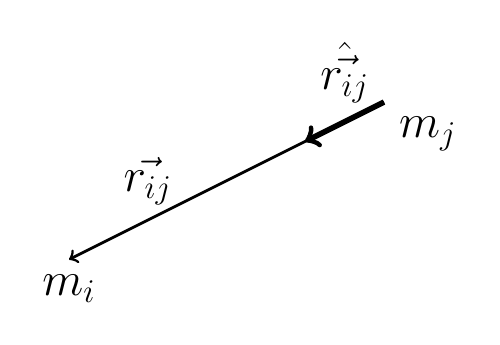
\begin{tikzpicture}
{\LARGE 
    \coordinate (a) at (0,0);
    \coordinate (ahat) at (3,1.5);
    \coordinate (b) at (4,2);
    \draw[->,line width=1] (b) to (a);
    \draw[->,line width=2] (b) to (ahat);
    \node[above right] at (0.5,.5) {$ \vec{r_{ij}} $};
    \node[above right] at (3,1.8) {$ \hat{\vec{r_{ij}}} $};
    \node[below] at (a) {$m_i$};
    \node[below right] at (b) {$m_j$};
}
\end{tikzpicture}
\end{center}

\begin{center}
{\LARGE $\vec{F_{ij}} = \left(G \frac{m_i m_j}{ |\vec{r_{ij}}|^2 }\right)\hat{\vec{r_{ij}}}$ }
\end{center}
\end{frame}

\begin{frame}[fragile,label=sec-25]{Bodies in Ruby}
 \begin{block}{the Body class should have a read-only mass}
\end{block}
\begin{block}{along with a position and a velocity}
\begin{minted}[]{ruby}
class Body
  attr_reader :mass
  attr_accessor :position, :velocity

  def initialize(mass:, position:, velocity:)
    @mass = mass
    @position = Vector.new(position)
    @velocity = Vector.new(velocity)
  end
end
\end{minted}
\end{block}
\end{frame}

\begin{frame}[fragile,label=sec-26]{Forces on Bodies in Ruby}
 \begin{block}{Bodies have a method to compute the gravitational force acting on it from another Body.}
\begin{minted}[]{ruby}
class Body
  def force_from(body)
    rvec = body.position - position
    r = rvec.norm
    rhat = rvec * (1/r)
    rhat * (Newtonian.G * mass * body.mass / r**2)
  end
end
\end{minted}
\end{block}
\end{frame}
\begin{frame}[label=sec-27]{the Universe}
\begin{quote}
It's very big \\
- Douglas Adams
\end{quote}
\end{frame}

\begin{frame}[fragile,label=sec-28]{the Universe in Ruby}
 \begin{block}{The final class will be Universe, it organizes all the bodies}
\begin{minted}[]{ruby}
class Universe
  attr_reader :dimensions, :bodies

  def initialize(dimensions:, bodies:)
    @dimensions = dimensions
    @bodies = bodies
  end
end
\end{minted}
\end{block}

\begin{block}{it also has a number of \alert{\alert{dimensions}}, we can use this to make sure the bodies are all in the same kind of space}
\end{block}
\end{frame}

\begin{frame}[fragile,label=sec-29]{the Enumerable Universe}
 \begin{block}{Since force is computed pairwise, we create an iterator for pairs of distinct objects}
\begin{minted}[]{ruby}
class Universe
  def each_pair_with_index
    bodies.each_with_index do |body_i, i|
      bodies.each_with_index do |body_j, j|
        next if i == j
        yield [body_i, body_j, i, j]
      end
    end
  end
end
\end{minted}
\end{block}
\end{frame}

\begin{frame}[fragile,label=sec-30]{The main simulation loop}
 \begin{minted}[]{ruby}
class Universe
  def evolve(dt)
    forces = bodies.map{ |_| zero_vector }
    each_pair_with_index do |(body_i, body_j, i, j)|
      forces[i] += body_i.force_from(body_j)
    end
    bodies.each_with_index do |_, i|
      a = forces[i] * (1.0 / bodies[i].mass)
      v = bodies[i].velocity 
      bodies[i].velocity += a * dt
      bodies[i].position += v * dt
    end
  end
end
\end{minted}
\end{frame}
\begin{frame}[label=sec-31]{The server}
\begin{block}{We can serve this up to a browser using}
\begin{itemize}
\item WEBrick for HTTP
\item websocketd for piping STDOUT to a WebSocket server
\end{itemize}
\end{block}
\end{frame}
\begin{frame}[fragile,label=sec-32]{Fork off an HTTP server}
 \begin{minted}[]{ruby}
rd, wt = IO.pipe
pid = fork do
  rd.close
  server = WEBrick::HTTPServer.new({
    :Port => PORT,
    :BindAddress => "localhost",
    :StartCallback => Proc.new {
      wt.write(1)  # write "1", signal start
      wt.close
    }
  })
  trap('INT') { server.stop }
  server.mount("/", WEBrick::HTTPServlet::FileHandler, './examples')
  server.start
end
# ...
\end{minted}
\end{frame}

\begin{frame}[fragile,label=sec-33]{Shell out to websocketd}
 \begin{block}{websocketd converts standard input and output into a fully functioning websocket server, so we can just puts out the universe state}
\begin{minted}[]{ruby}
examples = ["binary.rb", "ternary.rb", "random.rb", "figure_eight.rb"]
index = ARGV.last.to_i
# Shell out to websocketd, block until program finishes
system("bin/websocketd \
   -port=8080 \
   ruby #{examples[index]}")

Process.kill('INT', pid)   # kill HTTP server in child process
\end{minted}
\end{block}
\end{frame}

\begin{frame}[label=sec-34]{Binary Star system}
\begin{block}{Our first application is going to be simulating a binary star system, with two equal-mass stars}
\begin{center}
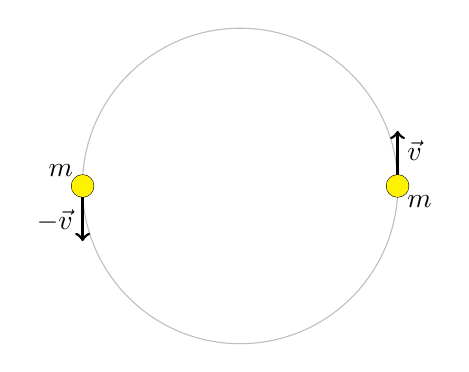
\begin{tikzpicture}
\coordinate (a) at (-2,0);
\coordinate (a') at (-2,-.7);
\coordinate (b) at (2,0);
\coordinate (b') at (2,.7);
\coordinate (c) at (0,0);
\draw[lightgray] (c) circle  (57pt);

\draw[->,line width=1] (a) to (a');
\draw[black] (a) circle (4pt);
\fill[yellow] (a) circle (4pt);
\node[above left] at (a) {$m$};
\node[above left] at (a') {$-\vec{v}$};

\draw[->,line width=1] (b) to (b');
\draw[black] (b) circle (4pt);
\fill[yellow] (b) circle (4pt);
\node[below right] at (b) {$m$};
\node[below right] at (b') {$\vec{v}$};

\end{tikzpicture}
\end{center}
\end{block}
\end{frame}
\begin{frame}[label=sec-35]{Find initial conditions}
\begin{block}{The two bodies will be traveling in uniform circular motion, so the following relation holds:}
\begin{center}
{\LARGE ${\color{red} a} = \frac{v^2}{r}$}

\begin{tikzpicture}
\coordinate (c) at (0pt,0pt);
\coordinate (p) at (75pt,0pt);
\coordinate (p') at (75pt,50pt);
\coordinate (m) at (50pt,0pt);

\draw[lightgray] (c) circle (75pt);
\draw[black] (p) circle (5pt);
\draw[->,line width=1] (p) to (p');
\draw[blue] (c) to (p);
\node[below left] at (30pt,0) {$r$};
\fill[white] (p) circle (5pt);
\node[below right] at (p') {$\vec{v}$};
\node[above right] at (p) {$|\vec{v}| = v$};
\node[below right,red] at (p) {$|\vec{a}| = a$ (centripetal acceleration)};

\draw[->,red,line width=1] (p) to (m);
\node[below,red] at (m) {$\vec{a}$};
\end{tikzpicture}
\end{center}
\end{block}
\end{frame}

\begin{frame}[label=sec-36]{Given the masses and the distance $r$, we can figure out $a$:}
\begin{center}
{\LARGE $ a = (Gm^2/4r^2)/m = Gm/4r^2 $}
\end{center}
\end{frame}
\begin{frame}[label=sec-37]{Substituting a back in to get $v$}
\begin{center}
{\LARGE $v = \sqrt{(Gm/4r^2)*r} = \sqrt{Gm/4r} $ }
\end{center}
\end{frame}
\begin{frame}[label=sec-38]{Run simulated binary star system}
\begin{block}{Pause to run simulations}
\end{block}
\end{frame}
\begin{frame}[label=sec-39]{The Three Body Problem}
\begin{block}{With only two bodies, it turns out to be possible to solve the equations of motion for \alert{all time}, exactly.}
\end{block}
\begin{block}{With three or more bodies, it is in general impossible}
\end{block}
\end{frame}
\begin{frame}[label=sec-40]{However}
\begin{block}{The three body problem has been studied since 1747, and there are some well known examples}
\end{block}
\end{frame}
\begin{frame}[label=sec-41]{The "Figure Eight" Three Body Orbit}
\begin{block}{The paper "A remarkable periodic solution of the three-body problem in the case of equal masses" by Alain Chenciner and Richard Montgomery works out an orbit that looks like this:}
\begin{center}
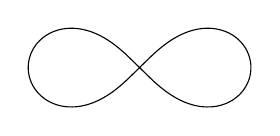
\begin{tikzpicture}
  \def\samples{100}
  \def\c{1}
  \pgfmathsetmacro\cc{\c*\c}
  \pgfmathsetmacro\cccc{\cc*\cc}
  \def\a{1.01}
  \draw
    (0, 0) --
    plot[
      variable=\t,
      domain=-45+1/\samples:45-1/\samples,
      samples=\samples,
      smooth,
    ]
    (\t:{\cc*sqrt(\cc*cos(2*\t) + \cc*cos(2*\t))})
    -- cycle
  ;
  \draw
    (0, 0) --
    plot[
      variable=\t,
      domain=180-45+1/\samples:180+45-1/\samples,
      samples=\samples,
      smooth,
    ]
    (\t:{\cc*sqrt(\cc*cos(2*\t) + \cc*cos(2*\t))})
    -- cycle
  ;
  \path plot coordinates { (-\c, 0) (\c, 0) };

\end{tikzpicture}
\end{center}
\end{block}
\end{frame}
\begin{frame}[label=sec-42]{The initial conditions}
\begin{block}{$\vec{x_1} = [0.97000436, -0.24308753]; \vec{x_2} = -\vec{x_1}$}
\end{block}
\begin{block}{$\vec{x_3} = \vec{0}$}
\end{block}
\begin{block}{$\vec{v_3} = [-0.93240737, -0.86473146]$}
\end{block}
\begin{block}{$-2\vec{v_1} = -2\vec{v_2} = \vec{v_3}$}
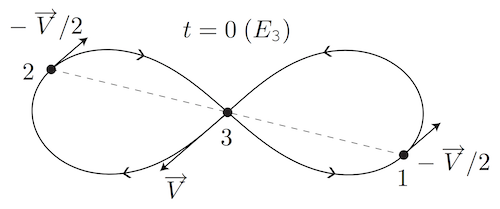
\includegraphics[width=.9\linewidth]{figure8.png}
\end{block}
\end{frame}
\begin{frame}[label=sec-43]{Run simulated three-body orbit}
\begin{block}{Pause to run simulations}
\end{block}
\end{frame}
% Emacs 24.5.1 (Org mode 8.2.10)
\end{document}
